\subsection{Live replay through the SDN}
\label{sec:replay}
Phase~B loaded the 10-client, seed-42 bundle and replayed each of the 14 attack captures from host $h_1$ (Table~\ref{tab:phaseb}). Every replay ended in a block decision, and the rule \texttt{priority=100,ip,nw\_src=10.0.0.1 actions=drop} was read back from the switch each time. Twelve of the 14 captures were given the right attack type, all by the booster. The MITM capture was called Ransomware, with only 542 of its 1,229 packets flagged. The OS-fingerprinting capture was called DDoS\_ICMP. Both are still blocked. The replays took 8 to 268~s, the longest for the 3.2-million-packet DDoS\_UDP capture.

Two facts limit what this shows. The captures are the dataset's own, so their rows are in the training data and the replay is a demonstration of the pipeline, not a held-out test. And the drop rule appears only after \texttt{tshark} has processed the whole capture: when it was read back, it had matched no packets, because the replay had already finished. Phase~B is batch classification of a capture, not inline blocking.

\begin{table*}[t]
\centering
\caption{Phase~B on every attack capture (10-client, seed-42 bundle). Confidence is the mean over the non-benign packets of the chosen label. All verdicts came from the booster.}
\label{tab:phaseb}
\small
\begin{adjustbox}{max width=\linewidth}
\begin{tabular}{llcrcr}
\toprule
Capture & Classified as & Confidence & Packets flagged & Action & Wall time (s) \\
\midrule
Backdoor attack & Backdoor & 0.997 & 24,543 / 24,914 & block & 12 \\
DDoS HTTP flood & DDoS\_HTTP & 0.966 & 119,748 / 229,142 & block & 29 \\
DDoS ICMP flood & DDoS\_ICMP & 1.000 & 2,914,156 / 2,914,356 & block & 232 \\
DDoS TCP SYN flood & DDoS\_TCP & 0.999 & 2,020,023 / 2,020,152 & block & 211 \\
DDoS UDP flood & DDoS\_UDP & 0.999 & 2,899,758 / 3,215,732 & block & 268 \\
MITM ARP spoofing + DNS & \textit{Ransomware} & 0.991 & 542 / 1,229 & block & 8 \\
OS fingerprinting & \textit{DDoS\_ICMP} & 0.980 & 1,134 / 1,176 & block & 9 \\
Password attacks & Password & 0.957 & 919,469 / 1,053,893 & block & 130 \\
Port scanning & Port\_Scanning & 0.999 & 22,495 / 23,329 & block & 12 \\
Ransomware & Ransomware & 0.994 & 10,620 / 11,030 & block & 11 \\
SQL injection & SQL\_injection & 1.000 & 51,097 / 51,228 & block & 17 \\
Uploading & Uploading & 0.999 & 37,592 / 37,644 & block & 15 \\
XSS & XSS & 0.999 & 15,677 / 16,215 & block & 12 \\
Vulnerability scanner & Vulnerability\_scanner & 0.996 & 262,922 / 265,827 & block & 60 \\
\bottomrule
\end{tabular}
\end{adjustbox}
\end{table*}

\subsection{Features for the first stage}
\label{sec:featstudy}
Table~\ref{tab:feat} follows LightGBM from the 91 base features to the full 130 on all rows. On the connection-grouped split, macro F1 rises from 0.889 to 0.924 with the service port, stays level with the content features, and jumps to 0.981 with the connection features. Content features add little on their own, because few packets carry content, but they feed the connection aggregates. Class weights bring the final configuration to 0.983, with accuracy 0.997. The ambiguity ceiling rises from 0.969 to 0.9997 macro recall, and the share of rows whose feature vector also occurs with another label falls from 2.31\% to 0.01\%. The random and grouped splits differ by at most 0.007 in macro F1 for every feature set, so neither feature set was relying on memorised connections.

\begin{table}[t]
\centering
\caption{LightGBM on all rows, seed 42, from the base features to the final 130. Random = rows split at random; grouped = connections held out. The ceiling is the best accuracy and macro recall any classifier on that feature set could reach.}
\label{tab:feat}
\small
\setlength{\tabcolsep}{2.5pt}
\begin{adjustbox}{max width=\linewidth}
\begin{tabular}{lrrcccccc}
\toprule
 & & & \multicolumn{2}{c}{Random} & \multicolumn{2}{c}{Grouped} & \multicolumn{2}{c}{Ceiling} \\
\cmidrule(lr){4-5}\cmidrule(lr){6-7}\cmidrule(lr){8-9}
Features & Count & Rows & Acc. & F1 & Acc. & F1 & Acc. & Rec. \\
\midrule
Base (authors' recipe) & 91 & 1,909,719 & 0.9638 & 0.8868 & 0.9637 & 0.8892 & 0.9875 & 0.9692 \\
+ service port & 92 & 1,909,980 & 0.9802 & 0.9245 & 0.9803 & 0.9236 & 0.9985 & 0.9940 \\
+ content & 110 & 1,909,980 & 0.9802 & 0.9268 & 0.9802 & 0.9232 & 0.9985 & 0.9940 \\
+ connection & 130 & 1,985,768 & 0.9977 & 0.9879 & 0.9975 & 0.9808 & 0.9999 & 0.9997 \\
+ class weights & 130 & 1,985,768 & 0.9976 & 0.9867 & 0.9972 & 0.9828 & 0.9999 & 0.9997 \\
\bottomrule
\end{tabular}
\end{adjustbox}
\end{table}

Fig.~\ref{fig:f1} shows where the gain comes from. The application-layer classes that the base features could not separate (Fingerprinting, Uploading, DDoS\_HTTP, SQL\_injection, Password and XSS) rise from 0.68--0.85 F1 to 0.93--1.00. Of the 1,113 remaining errors at seed 42, 54\% are Password and DDoS\_HTTP confused with each other, both HTTP requests to the same server, and 14\% are Ransomware and Backdoor confused with each other (Fig.~\ref{fig:cm}).

\begin{figure}[t]
\centering
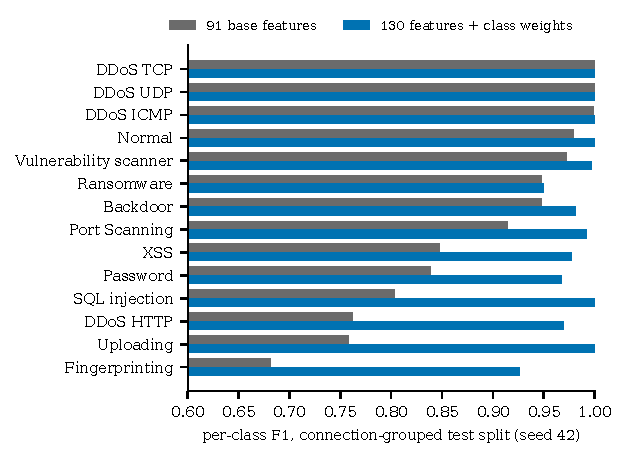
\includegraphics[width=\columnwidth]{figs/fig_f1.pdf}
\caption{Per-class F1 of LightGBM with the 91 base features and with the final 130 features and class weights, connection-grouped split, seed 42. MITM cannot be scored on this split.}
\label{fig:f1}
\end{figure}

\begin{figure}[t]
\centering
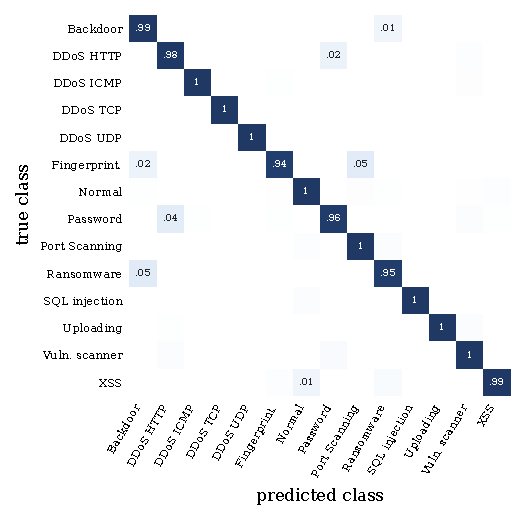
\includegraphics[width=\columnwidth]{figs/fig_cm.pdf}
\caption{Confusion matrix of the final classifier (130 features, class weights), connection-grouped test split, seed 42, row-normalised. Shading is stretched (square-root scale) so that small errors are visible.}
\label{fig:cm}
\end{figure}

Table~\ref{tab:seeds} repeats the final configuration over three seeds. Grouped macro F1 is 0.983, 0.984 and 0.985. Without class weights it swings from 0.981 to 0.952, because Fingerprinting, with few connections, varies widely. The same configuration trained on only 5\% of the rows, the size of the calibration set, reaches 0.997 accuracy and 0.979 macro F1 on the same grouped test set, against 0.962 and 0.881 for the base features under the same restriction. So the bootstrap booster in the federated system is not much weaker for training on the server's small set.

Two of the added features owe part of their value to the testbed. Benign traffic in Edge-IIoTset is MQTT and VNC and never HTTP, so a service port of 80 alone hints at an attack. In a network with benign web traffic, that feature would separate much less. The keyword groups were chosen with the dataset's attack families in mind, which makes them closer to signatures than to general behaviour.

\textit{Time-ordered split.} Training on each class's earlier connections and testing on its later ones gives 0.994 accuracy and 0.912 to 0.913 macro F1 over three seeds (Table~\ref{tab:seeds}). The lower macro F1 is mostly an artifact. MITM is one connection, so this split puts it entirely in the test side, where its recall of 0 enters the mean of 15 classes. Without MITM, the seed-42 macro F1 would be about 0.978. The real losses are on Backdoor (recall 0.947 to 0.962, against 0.989 on the grouped split) and DDoS\_HTTP (0.912 to 0.925, against 0.980).

\begin{table}[t]
\centering
\caption{Final classifier configuration across seeds: random split, grouped split, grouped split without class weights, and time-ordered split.}
\label{tab:seeds}
\small
\setlength{\tabcolsep}{3pt}
\begin{adjustbox}{max width=\linewidth}
\begin{tabular}{rcccccc}
\toprule
 & Random & \multicolumn{2}{c}{Grouped} & Grouped, no weights & \multicolumn{2}{c}{Time-ordered} \\
\cmidrule(lr){2-2}\cmidrule(lr){3-4}\cmidrule(lr){5-5}\cmidrule(lr){6-7}
Seed & F1 & Acc. & F1 & F1 & Acc. & F1 \\
\midrule
42 & 0.9867 & 0.9972 & 0.9828 & 0.9808 & 0.9942 & 0.9133 \\
43 & 0.9868 & 0.9971 & 0.9835 & 0.9560 & 0.9943 & 0.9122 \\
44 & 0.9866 & 0.9970 & 0.9851 & 0.9521 & 0.9941 & 0.9129 \\
\bottomrule
\end{tabular}
\end{adjustbox}
\end{table}

\subsection{Communication, training time and decision time}
The autoencoder's 9,834 float32 parameters cost $2\times9{,}834\times4=78{,}672$ bytes per client per round, downlink plus uplink: 786,720 bytes per round for 10 clients and 15,734,400 over 20 rounds. That figure leaves out the booster, which the server sends to every client every round. Its serialised file is 8.9 to 10.4~MB across the six runs, so one client's copy alone is more than ten times a whole round of autoencoder traffic for ten clients. Sending it only when its version changes, at most every third round, is a simple saving we have not implemented.

We timed the cascade on the saved 10-client, seed-42 bundle, one CPU thread of the VM's Intel Xeon, with 3,000 held-out test packets timed one call each and one batch of 200,000. The classifier alone takes a median 0.372~ms per packet (95th percentile 0.440), the autoencoder alone 0.060~ms (0.094), and both stages 0.642~ms (0.706). In batch mode the cascade handles 3,760 packets per second, 265.9~$\mu$s per packet, almost all of it in the booster (the autoencoder alone takes 5.5~$\mu$s). These are model times only: they exclude reading a capture, \texttt{tshark} feature extraction and the switch, and they come from one bundle on one machine, so we claim no confidence interval.
